
%(BEGIN_QUESTION)
% Copyright 2010, Tony R. Kuphaldt, released under the Creative Commons Attribution License (v 1.0)
% This means you may do almost anything with this work of mine, so long as you give me proper credit

Sketch connecting wires to allow this data acquisition unit (DAQ) to sense current (using the ``shunt'' resistor as a primary sensing element) on input channel \#2 and also generator output voltage on input channel \#3:

$$\includegraphics[width=15.5cm]{i04583x01.eps}$$

Your circuit should be wired in such a way that a {\it discharging} battery produces a {\it negative} signal at channel \#2, and a {\it charging} battery produces a {\it positive} signal at channel \#2.  

\vfil 

\underbar{file i04583}
\eject
%(END_QUESTION)





%(BEGIN_ANSWER)

This is a graded question -- no answers or hints given!

%(END_ANSWER)





%(BEGIN_NOTES)

Each differential input on this DAQ should be treated like a voltmeter.  Just ask yourself, ``How would I connect a voltmeter to measure these quantities in the circuit?'' and this line of thought will guide your wire connections between the DAQ and the circuit under test.  Note also that a path for DAQ input bias currents must be provided, which explains the ``AI Gnd'' wire connecting to the grounded pole of the generator circuit:

$$\includegraphics[width=15.5cm]{i04583x02.eps}$$

A good problem-solving technique to apply here with respect to identifying the proper connections for channel \#2 is to draw the direction(s) of battery current, and use the arrow(s) to identify polarity of voltage across the shunt resistor.  When students miss this part of the question, it's usually because they did not take the time to sketch this detail and carefully check polarity.

%INDEX% Pictorial circuit review (analog signal wiring to data acquisition unit)

%(END_NOTES)

